\documentclass[tikz,border=12pt]{standalone}
\usepackage{tikz}
\usetikzlibrary{arrows.meta}

\definecolor{fairblue}{RGB}{33, 102, 172}
\definecolor{fairmidblue}{RGB}{103, 169, 207}
\definecolor{fairlight}{RGB}{247, 247, 247}
\definecolor{fairmidred}{RGB}{239, 138, 98}
\definecolor{fairred}{RGB}{178, 24, 43}
\definecolor{darkgray}{RGB}{60, 60, 60}
\definecolor{lightgrid}{RGB}{230, 230, 230}

\begin{document}
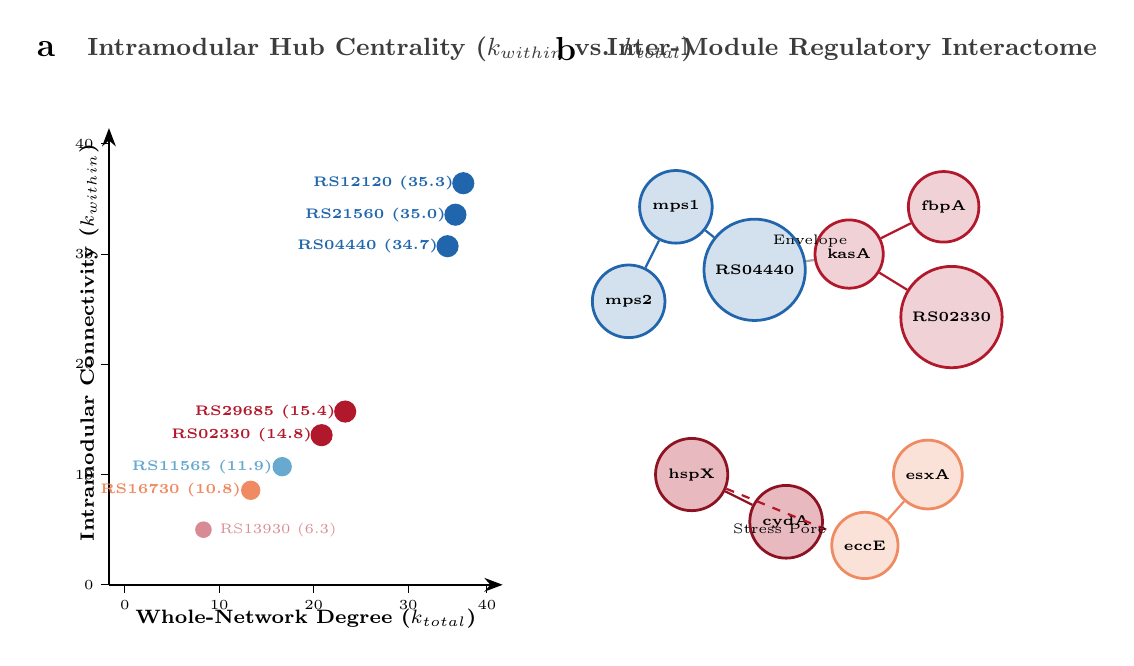
\begin{tikzpicture}[font=\sffamily, >=Stealth]
  % Panel a: Scatter Plot k_within vs k_total
  \node[font=\large\bfseries] at (0, 7.8) {a};
  \node[anchor=west, font=\small\bfseries, text=darkgray] at (0.4, 7.8) {Intramodular Hub Centrality ($k_{\text{within}}$ vs. $k_{\text{total}}$)};

  \draw[->, thick] (0.8, 1.0) -- (5.8, 1.0) node[midway, below=5pt, font=\scriptsize\bfseries] {Whole-Network Degree ($k_{\text{total}}$)};
  \draw[->, thick] (0.8, 1.0) -- (0.8, 6.8) node[midway, above=5pt, rotate=90, font=\scriptsize\bfseries] {Intramodular Connectivity ($k_{\text{within}}$)};

  \foreach \x/\lbl in {1.0/0, 2.2/10, 3.4/20, 4.6/30, 5.6/40} {
    \draw (\x, 0.9) -- (\x, 1.0) node[below=2pt, font=\tiny] {\lbl};
  }
  \foreach \y/\lbl in {1.0/0, 2.4/10, 3.8/20, 5.2/30, 6.6/40} {
    \draw (0.7, \y) -- (0.8, \y) node[left=2pt, font=\tiny] {\lbl};
  }

  % Hub Points
  \fill[fairblue] (5.3, 6.1) circle (4pt) node[anchor=east, font=\tiny\bfseries] {RS12120 (35.3)\ };
  \fill[fairblue] (5.2, 5.7) circle (4pt) node[anchor=east, font=\tiny\bfseries] {RS21560 (35.0)\ };
  \fill[fairblue] (5.1, 5.3) circle (4pt) node[anchor=east, font=\tiny\bfseries] {RS04440 (34.7)\ };

  \fill[fairred] (3.8, 3.2) circle (4pt) node[anchor=east, font=\tiny\bfseries] {RS29685 (15.4)\ };
  \fill[fairred] (3.5, 2.9) circle (4pt) node[anchor=east, font=\tiny\bfseries] {RS02330 (14.8)\ };

  \fill[fairmidblue] (3.0, 2.5) circle (3.5pt) node[anchor=east, font=\tiny\bfseries] {RS11565 (11.9)\ };
  \fill[fairmidred] (2.6, 2.2) circle (3.5pt) node[anchor=east, font=\tiny\bfseries] {RS16730 (10.8)\ };
  \fill[fairred!50!white] (2.0, 1.7) circle (3pt) node[anchor=west, font=\tiny] {\ RS13930 (6.3)};

  % Panel b: Regulatory Interactome
  \node[font=\large\bfseries] at (6.6, 7.8) {b};
  \node[anchor=west, font=\small\bfseries, text=darkgray] at (7.0, 7.8) {Inter-Module Regulatory Interactome};

  % Network Nodes
  \node[circle, fill=fairblue!20, draw=fairblue, line width=1pt, font=\tiny\bfseries] (mps1) at (8.0, 5.8) {mps1};
  \node[circle, fill=fairblue!20, draw=fairblue, line width=1pt, font=\tiny\bfseries] (mps2) at (7.4, 4.6) {mps2};
  \node[circle, fill=fairblue!20, draw=fairblue, line width=1pt, font=\tiny\bfseries] (rs04) at (9.0, 5.0) {RS04440};

  \node[circle, fill=fairred!20, draw=fairred, line width=1pt, font=\tiny\bfseries] (kasA) at (10.2, 5.2) {kasA};
  \node[circle, fill=fairred!20, draw=fairred, line width=1pt, font=\tiny\bfseries] (fbpA) at (11.4, 5.8) {fbpA};
  \node[circle, fill=fairred!20, draw=fairred, line width=1pt, font=\tiny\bfseries] (rs02) at (11.5, 4.4) {RS02330};

  \node[circle, fill=fairred!30, draw=fairred!80!black, line width=1pt, font=\tiny\bfseries] (hspX) at (8.2, 2.4) {hspX};
  \node[circle, fill=fairred!30, draw=fairred!80!black, line width=1pt, font=\tiny\bfseries] (cydA) at (9.4, 1.8) {cydA};

  \node[circle, fill=fairmidred!25, draw=fairmidred, line width=1pt, font=\tiny\bfseries] (esxA) at (11.2, 2.4) {esxA};
  \node[circle, fill=fairmidred!25, draw=fairmidred, line width=1pt, font=\tiny\bfseries] (eccE) at (10.4, 1.5) {eccE};

  % Edges
  \draw[thick, draw=fairblue] (mps1) -- (mps2);
  \draw[thick, draw=fairblue] (mps1) -- (rs04);
  \draw[thick, dashed, draw=gray!70] (rs04) -- (kasA) node[midway, above=1pt, font=\tiny] {Envelope};
  \draw[thick, draw=fairred] (kasA) -- (fbpA);
  \draw[thick, draw=fairred] (kasA) -- (rs02);
  \draw[thick, draw=fairred!80!black] (hspX) -- (cydA);
  \draw[thick, draw=fairmidred] (esxA) -- (eccE);
  \draw[thick, dashed, draw=fairred] (hspX) -- (eccE) node[midway, below=1pt, font=\tiny] {Stress Pore};
\end{tikzpicture}
\end{document}
